
\chapter{Angular Convolution, A Better Algorithm\label{chpt:angular-convolution}}

In previous sections, the spatial convolution in the excess functional
gradient is treated by \acs{FFT} thanks to the transitional invariance
that leads to $\mathbf{r}_{12}=\mathbf{r}_{1}-\mathbf{r}_{2}$. However,
as the angular grid is not homogeneous, the relative coordinates of
two angles cannot be simply represented $\mathbf{\Omega}_{12}=\mathbf{\Omega}_{1}-\mathbf{\Omega}_{2}$,
therefore for the angles we cannot take advantage of the convolution
property shown in eq. (\ref{eq:convolution-1}-\ref{eq:convolution-2}).
On the other hand, these two-particle quantities have rotational invariance.
As proposed by Blum \citep{Blum_I,Blum_II}, a rotational invariant
expansion technique is used to reduce the molecular Ornstein-Zernike
(\acs{MOZ}) equation into smaller irreducible matrix equations ($\mathsection$\ref{sec:Angular-dependent-iem}).
Owing to the mathematical equivalence between \acs{IET} and \acs{DFT}
approach ($\mathsection$\ref{sec:Equivalence-iet-mdft}), where eq.
(\ref{eq:gamma-k}) about the Fourier transform of the excess functional
gradient can be regarded as the \acs{MOZ} equation, the formalism
of Blum can also be applied to \acs{MDFT}.

\section{Angular convolution using Blum's reduction}

\marginpar{Here the projections $F_{\mu\nu,\chi}^{mn}$ are defined as in \citep{Fries_Patey_1985}.\textcolor{red}{{}
}Eq. (\ref{eq:Blum-reduced-OZ}) is mathematically identical with
those in \citep{Blum_I,Blum_II} but using $R_{\mu'\mu}^{m}=D_{\mu\mu'}^{m*}$.
The difference between the conventions of \acs{GSH} are listed in
$\mathsection$\ref{sec:Convention-of-GSH}.}To build an analogue of the irreducible form of \acs{MOZ} equation
for homogeneous fluid deduced by Blum (detailed in $\mathsection$\ref{sec:Angular-dependent-iem})
\begin{equation}
\hat{\gamma'}_{\lambda\mu,\chi}^{lm}(k)=\sum_{n=0}^{n_{\mathrm{max}}}\sum_{\nu=-n}^{n}\left(-\right){}^{\chi+\nu}\Delta\hat{\rho'}_{\lambda\underline{\nu},\chi}^{ln}(k)\hat{c'}_{\nu\mu,\chi}^{nm}(k)\label{eq:Blum-reduced-OZ}
\end{equation}
for the \acs{MDFT} formalism, a generalized spherical harmonic transform
(\acs{GSHT}) treatment is proposed by developing the functional gradient
$\hat{\gamma}$ and the density $\hat{\rho}$ in eq. (\ref{eq:gamma-k})
on Wigner generalized spherical harmonics (\acs{GSH}):
\begin{equation}
\hat{\gamma}(\mathbf{k},\mathbf{\Omega}_{1})=\sum_{m\mu'\mu}f_{m}\hat{\gamma}_{\mu'\mu}^{m}(\mathbf{k})R_{\mu'\mu}^{m}(\mathbf{\Omega}_{1})\label{eq:gamma-projection}
\end{equation}
\begin{equation}
\Delta\hat{\rho}(\mathbf{k},\mathbf{\Omega}_{2})=\sum_{n\nu'\nu}f_{n}\Delta\hat{\rho}_{\nu',\nu}^{n}(\mathbf{k})R_{\nu',\nu}^{n}(\mathbf{\Omega}_{2})\label{eq:delta-rho-projection}
\end{equation}
where $0\leq m,n\leq n_{\mathrm{max}}$, $\left|\mu'\right|,\left|\mu\right|\leq m$
and $\left|\nu'\right|,\left|\nu\right|\leq n$. $f_{m}=\left(2m+1\right)^{\frac{1}{2}}=\left\Vert R_{\mu'\mu}^{m}\right\Vert ^{-1}$
is the normalization factor.

The \acs{DCF} can also be expanded on rotational invariants:
\begin{equation}
\hat{c}(k,\mathbf{\Omega}_{1},\mathbf{\Omega}_{2})=\sum_{mnl\mu\nu}f_{m}f_{n}\hat{c}_{\mu\nu}^{mnl}(k)\sum_{\mu'\nu'\lambda'}\left(\begin{array}{ccc}
m & n & l\\
\mu' & \nu' & \lambda'
\end{array}\right)R_{\mu'\mu}^{m}(\mathbf{\Omega}_{1})R_{\nu'\nu}^{n}(\mathbf{\Omega}_{2})R_{\lambda'0}^{l}(\hat{\mathbf{k}})\label{eq:c-projection}
\end{equation}

As \acs{GSH} possess orthogonality eq. (\ref{eq:gsh-orthogonality})
and symmetry eq. (\ref{eq:symm-gsh-1}), eq. (\ref{eq:gamma-k}) can
be rewritten by (\ref{eq:gamma-projection}, \ref{eq:delta-rho-projection},
\ref{eq:c-projection}), which gives (here we omit the detailed demonstration
for simplicity, which is put in appendix \ref{chpt:deduction_blum}):
\begin{equation}
\hat{\gamma}_{\mu'\mu}^{m}(\mathbf{k})=\sum_{nl\nu}\hat{c}_{\mu\nu}^{mnl}(k)\sum_{\nu'\lambda'}\left(-\right){}^{\nu'+\nu}\Delta\hat{\rho}_{\underline{\nu'}\underline{\nu}}^{n}(\mathbf{k})\left(\begin{array}{ccc}
m & n & l\\
\mu' & \nu' & \lambda'
\end{array}\right)R_{\lambda'0}^{l}(\hat{\mathbf{k}})\label{eq:im}
\end{equation}
thus the \acs{OZ} equation is expanded on \acs{GSH}s and rotational
invariants.

Note that eq. (\ref{eq:im}) is reducible. Blum's $\chi$-transform
\citep{Blum_II} defines:
\begin{equation}
\hat{c'}_{\mu\nu,\chi}^{mn}(k)=\sum_{l=\left|m-n\right|}^{m+n}\left(\begin{array}{ccc}
m & n & l\\
\chi & -\chi & 0
\end{array}\right)\hat{c}_{\mu\nu}^{mnl}(k)
\end{equation}
\begin{equation}
\hat{c}_{\mu\nu}^{mnl}(k)=\left(2l+1\right)\sum_{\chi=-\min(m,n)}^{\min(m,n)}\left(\begin{array}{ccc}
m & n & l\\
\chi & -\chi & 0
\end{array}\right)\hat{c'}_{\mu\nu,\chi}^{mn}(k)\label{eq:c-p}
\end{equation}

Invariants of form $F_{\mu\nu,\chi}^{mn}(k)$ have a very simple relation
with their combined function $F(k,\boldsymbol{\omega_{1}},\boldsymbol{\omega_{2}})$
in intermolecular coordinate system (see appendix \ref{chpt:rotational-invariant-expansion},
eq. (\ref{eq:local-forward}, \ref{eq:local_backward})), that is
how the \acs{OZ} equation can be reduced. In \acs{MDFT}, we can
also take advantage of this quantity by defining the projections of
$\hat{\gamma}$ and $\hat{\rho}$ in the local frame ($\boldsymbol{\omega}_{i}=\hat{\mathbf{k}}^{-1}\mathbf{\Omega}_{i}$):
\begin{equation}
\hat{\gamma}(\mathbf{k},\boldsymbol{\omega}_{1})=\sum_{m\chi\mu}f_{m}\hat{\gamma'}_{\chi\mu}^{m}(\mathbf{k})R_{\chi\mu}^{m}(\boldsymbol{\omega}_{1})\label{eq:gamma-projection-local}
\end{equation}
\begin{equation}
\Delta\hat{\rho}(\mathbf{k},\boldsymbol{\omega}_{2})=\sum_{n\chi\nu}f_{n}\Delta\hat{\rho'}_{\chi\nu}^{n}(\mathbf{k})R_{\chi\nu}^{n}(\mathbf{\boldsymbol{\omega}}_{2})\label{eq:delta-rho-projection-local}
\end{equation}
and with the rotation formula of \acs{GSH} (eq. (\ref{eq:gsh-rotation})),
we have 
\begin{equation}
\hat{\gamma'}_{\chi\mu}^{m}(\mathbf{k})=\sum_{\mu'}\hat{\gamma}_{\mu'\mu}^{m}(\mathbf{k})R_{\mu'\chi}^{m}(\hat{\mathbf{k}})\label{eq:gamma-p}
\end{equation}
\begin{equation}
\Delta\hat{\rho}_{\underline{\nu'}\underline{\nu}}^{n}(\mathbf{k})=\sum_{\chi}\Delta\hat{\rho'}_{\chi\underline{\nu}}^{n}(\mathbf{k})R_{\underline{\nu'}\chi}^{n*}(\hat{\mathbf{k}})=\sum_{\chi}\Delta\hat{\rho'}_{\chi\underline{\nu}}^{n}(\mathbf{k})\left(-\right){}^{\chi+\nu'}R_{\nu'\underline{\chi}}^{n}(\hat{\mathbf{k}})\label{eq:rho-p}
\end{equation}

Using eq. (\ref{eq:im}), (\ref{eq:c-p}), (\ref{eq:gamma-p}), (\ref{eq:rho-p})
and \acs{GSH} products relation eq. (\ref{eq:gg.a91}) and 3j-symbol
orthogonality eq. (\ref{eq:3j-orthogonality}), we deduce that:\marginpar{This \acs{OZ} equation formalism is the main result of the new theory.
A step-by-step operational way to make use of this equation for $\gamma$
evaluation is shown in $\mathsection$\ref{sec:Operational-algorithm}.}
\begin{equation}
\hat{\gamma'}_{\chi\mu}^{m}(\mathbf{k})=\sum_{n\nu}\left(-\right){}^{\chi+\nu}\hat{c'}_{\mu\nu,\chi}^{mn}(k)\Delta\hat{\rho'}_{\chi\underline{\nu}}^{n}(\mathbf{k})\label{eq:gamma-blum}
\end{equation}

Eq. (\ref{eq:gamma-blum}) is essential to the new algorithm. It makes
that, for the terms with the same index $\chi$, the \acs{OZ} equation
is a simple product of matrix:
\begin{equation}
\tilde{\gamma'}_{\chi}=\left[\left(-\right){}^{\chi+\nu}\tilde{c'}_{\chi}\right]\tilde{\rho'}_{\chi}
\end{equation}

The index $\chi$ shares the same role with $\mathbf{k}$ in the treatment
of spatial convolution, where the recombination of projections on
the exponential orthogonal bases gives for each $\mathbf{k}$, a simple
product form of the \acs{OZ} equation.

If we consider the solute is the same as solvent, and take $\hat{c'}_{\nu\mu,\underline{\chi}}^{nm}(k)$
in the place of $\hat{c'}_{\mu\nu,\chi}^{mn}(k)$, eq. (\ref{eq:gamma-blum})
is mathematically identical to eq. (\ref{eq:Blum-reduced-OZ}), as:
\begin{equation}
\hat{\gamma'}_{\chi\mu}^{m}(\mathbf{k})=\sum_{l\lambda}f^{l}\hat{\gamma'}_{\lambda\mu,\underline{\chi}}^{lm}(k)R_{\underline{\chi}\lambda}^{l}(\hat{\mathbf{k}})
\end{equation}
\begin{equation}
\hat{\rho'}_{\chi\underline{\nu}}^{n}(\mathbf{k})=\sum_{l\lambda}f^{l}\Delta\hat{\rho'}_{\lambda\underline{\nu},\underline{\chi}}^{ln}(k)R_{\underline{\chi}\lambda}^{l}(\hat{\mathbf{k}})
\end{equation}
according to the rotational invariant transform in eq. (\ref{eq:local-forward}).
In fact, it can be proven (with $\mathsection$\ref{sec:Symmetry-rot_invar})
that:
\begin{equation}
\hat{c'}_{\nu\mu,\underline{\chi}}^{nm}(k)=\hat{c'}_{\mu\nu,\chi}^{mn*}(k)
\end{equation}
The incompatibility in the conjugate is yet to be understand. In the
code, when we use the $\hat{c'}_{\mu\nu,\chi}^{mn}(k)$ issued from
\acs{IET}, we also need to take its conjugate to obtain the same
result as \acs{IET}. Note that the demonstration from eq. (\ref{eq:gamma-projection})
to eq. (\ref{eq:gamma-blum}) does not contain any incompatibility,
it only occurs in the comparison with the \acs{IET} formalism for
homogeneous liquids.

With the approach described above, the integral of the angular part
in eq. (\ref{eq:gamma-k}) can be reduced to a sum of a few terms.
Table \ref{tab:FE-of-OZ} shows some parameters linking to computing
cost of different algorithms. \marginpar{\protect\textsuperscript{{*}}Only if we do not need to calculate
$\hat{c}(\mathbf{k},\mathbf{\Omega}_{1},\mathbf{\Omega}_{2})$.}It shows that the expansion on \acs{GSH}s (eq. (\ref{eq:im})) does
not give any reduction of \acs{FE} compared to its 6D function form
(eq. (\ref{eq:gamma-k}))\textsuperscript{{*}}; but after the Blum's
$\chi$-transform, the \acs{OZ} equation is largely reduced. The
fact is that as the treatment of spatial convolution takes advantage
of the transitional invariance $r_{12}$, the $\chi$-transform makes
use of the rotational invariance.

\begin{table}[t]
\centering{}\hspace{0em} %
\noindent\begin{minipage}[t]{1\columnwidth}%
\begin{center}
\begin{tabular*}{1\textwidth}{@{\extracolsep{\fill}}ccccccc}
\toprule 
\addlinespace[-0.17em]
{\scriptsize{}$m_{\mathrm{max}}$} & {\scriptsize{}0} & {\scriptsize{}1} & {\scriptsize{}2} & {\scriptsize{}3} & {\scriptsize{}4} & {\scriptsize{}5}\tabularnewline
\midrule 
\addlinespace[-0.33em]
{\scriptsize{}$N_{\Theta}$} & {\scriptsize{}1} & {\scriptsize{}2} & {\scriptsize{}3} & {\scriptsize{}4} & {\scriptsize{}5} & {\scriptsize{}6}\tabularnewline
\addlinespace[-0.33em]
{\scriptsize{}$N_{\mathrm{ang}}$ (Gauss-Legendre)} & {\scriptsize{}1 (1)} & {\scriptsize{}18 (6)} & {\scriptsize{}75 (45)} & {\scriptsize{}196 (84)} & {\scriptsize{}405 (225)} & {\scriptsize{}726 (330)}\tabularnewline
\addlinespace[-0.33em]
{\scriptsize{}$N_{\mathrm{ang}}$ (Lebedev$\times\psi$)} & {\scriptsize{}1 (1)} & {\scriptsize{}18 (6)} & {\scriptsize{}70 (42)} & {\scriptsize{}182 (78)} & {\scriptsize{}342 (190)} & {\scriptsize{}550 (250)}\tabularnewline
\addlinespace[-0.33em]
{\scriptsize{}$N_{\mathrm{proj}}$ } & {\scriptsize{}1 (1)} & {\scriptsize{}10 (4)} & {\scriptsize{}35 (19)} & {\scriptsize{}84 (40)} & {\scriptsize{}165 (85)} & {\scriptsize{}286 (140)}\tabularnewline
\addlinespace[-0.33em]
{\scriptsize{}FE for eq. (\ref{eq:gamma-k})} & {\scriptsize{}1 (1)} & {\scriptsize{}324 (36)} & {\scriptsize{}5625 (2025)} & {\scriptsize{}38416 (7056)} & {\scriptsize{}164025 (50625)} & {\scriptsize{}527076 (108900)}\tabularnewline
\addlinespace[-0.33em]
{\scriptsize{}FE for eq. (\ref{eq:im})} & {\scriptsize{}1 (1)} & {\scriptsize{}262 (34)} & {\scriptsize{}4787 (1459)} & {\scriptsize{}36588 (8116)} & {\scriptsize{}175989 (47221)} & {\scriptsize{}633490 (150566)}\tabularnewline
\addlinespace[-0.33em]
{\scriptsize{}FE for eq. (\ref{eq:gamma-blum})} & {\scriptsize{}1 (1)} & {\scriptsize{}34 (6)} & {\scriptsize{}259 (75)} & {\scriptsize{}1092 (252)} & {\scriptsize{}3333 (877)} & {\scriptsize{}8294 (2002)}\tabularnewline
\bottomrule
\end{tabular*}\caption[Number of FE needed by OZ equation of different form]{Number of \acs{FE} needed by \acs{OZ} equation of different form
for arbitrary solvent (outside the parentheses) and solvent possessing
$\mathrm{C}_{2v}$ symmetry (inside the parentheses)\label{tab:FE-of-OZ}}
\par\end{center}%
\end{minipage}
\end{table}


\section{Fast generalized spherical harmonic transform\label{sec:fgsht}}

The algorithm above for angular convolution takes advantage of the
orthogonality and symmetries of \acs{GSH}s. To use this algorithm
as analogous to the treatment of the convolution with \acs{FFT} for
spatial grids, the transform described in eq. (\ref{eq:gamma-projection})
and (\ref{eq:delta-rho-projection}), here defined as the generalized
spherical harmonic transform (\acs{GSHT}), \textit{a priori }should
be fast. This is possible owing to the exponential components in the
definition of \acs{GSH}, that will be discussed later as the fast
generalized spherical harmonic transform (\acs{FGSHT}).

\acs{GSHT} provides a forward-backward transform between a general
angular function $F(\mathbf{\Omega})\equiv F(\cos\Theta,\Phi,\Psi)$
and its projections $F_{\mu'\mu}^{m}$ ($\left|\mu'\right|,\left|\mu\right|\leq m$):
\begin{equation}
F_{\mu'\mu}^{m}=\frac{f_{m}}{8\pi^{2}}\int\mathrm{d}\mathbf{\Omega}F(\mathbf{\Omega})R_{\mu'\mu}^{m*}(\mathbf{\Omega})\begin{array}{c}
\mathrm{(forward)}\end{array}\label{eq:GSHT_forward}
\end{equation}
\begin{equation}
F(\mathbf{\Omega})=\sum_{m,\mu',\mu}f_{m}F_{\mu'\mu}^{m}R_{\mu'\mu}^{m}(\mathbf{\Omega})\begin{array}{c}
\mathrm{(backward)}\end{array}\label{eq:GSHT_backward}
\end{equation}
where $\left\{ R_{\mu'\mu}^{m}(\mathbf{\Omega})\right\} $ are the
Wigner generalized spherical harmonics (Appendix \ref{chpt:symmetry}),
which form a complete orthogonal set, being defined as:
\begin{equation}
R_{\mu'\mu}^{m}(\mathbf{\Omega})=r_{\mu'\mu}^{m}(\Theta)e^{-i(\mu'\Phi+\mu\Psi)}
\end{equation}


\subsection{Equivalence of order in angular quadratures and projections}

Suppose that $F(\mathbf{\Omega})$ is a polynomial of both $\cos\Theta$,
$\cos\Phi$ and $\cos\Psi$ of order $n$, ($n+1$ polynomial terms).
To completely expand this function as shown in equation (\ref{eq:GSHT_backward}),
at least $m_{\mathrm{max}}=n$ is needed, where $m_{\mathrm{max}}$
is the highest order of projections $F_{\mu'\mu}^{m}$ in the expansion.
Note that $m_{\mathrm{max}}=n$ is not always sufficient to completely
expand $F(\mathbf{\Omega})$, a discussion to this issue will be given
in $\mathsection$\ref{sec:gsh-imp}. 

To evaluate exactly the integration in equation (\ref{eq:GSHT_forward}),
at least $n+1$ for $\cos\Theta$ (Gauss-Legendre grid), $2n+1$ for
$\Phi$ (equal-spaced grid), $2n+1$ for $\Psi$ (equal-spaced grid)
points of angular grid are needed (c.f. appendix \ref{chpt:equivalence-of-quadrature-projection-order}).
In the case of water which possesses a $\mathrm{C}_{2}$ symmetry
$F(\Psi+\pi)=F(\Psi)$, only projections of even $\mu$ are nonzero:
\begin{eqnarray}
F_{\mu} & = & \int\mathrm{d}\Psi F(\Psi)e^{i\mu\Psi}=\int\mathrm{d}(\Psi+\pi)F(\Psi+\pi)e^{i\mu(\Psi+\pi)}\nonumber \\
 & = & e^{i\mu\pi}\int\mathrm{d}\Psi F(\Psi)e^{i\mu\Psi}=e^{i\mu\pi}F_{\mu}
\end{eqnarray}

\begin{equation}
F_{\mu}=\begin{cases}
0 & \mu=2n+1,n\in\mathbb{Z}\\
F_{\mu} & \mu=2n,n\in\mathbb{Z}
\end{cases}
\end{equation}

Therefore the function
\begin{equation}
F(\Psi)=\sum_{\mu}F_{\mu}e^{-i\mu\Psi}
\end{equation}
can be rewritten as:
\begin{equation}
F(\Psi_{2}/2\equiv\Psi)=\sum_{\mu_{2}\equiv\mu/2}F_{2\mu_{2}}e^{-i\mu_{2}\Psi_{2}}
\end{equation}

As $\left|\mu_{2}\right|\leq n/2$, $F(\Psi_{2}/2\equiv\Psi)$ is
a polynomial of $\cos\Psi_{2}$ of order $\mathrm{floor}(n/2)\equiv\left\lfloor n/2\right\rfloor $,
in the forward transform
\begin{equation}
F_{2\mu_{2}\equiv\mu}=\intop\mathrm{d}\Psi F(\Psi)e^{i\mu\Psi}=\frac{1}{2}\intop\mathrm{d}\Psi_{2}F(\Psi_{2}/2\equiv\Psi)e^{i\mu_{2}\Psi_{2}}
\end{equation}
the total degree $\cos\Psi_{2}$ polynomial in the integrand is $2\left\lfloor n/2\right\rfloor $,
then $2\left\lfloor n/2\right\rfloor +1$ points of $\Psi_{2}$ (or
$\Psi$) are needed. 

For further implementation, we take these conclusions, but distinguish
the order of quadrature $m_{\mathrm{max}}$ (linked to the angular
grid) and the order of projection $n_{\mathrm{max}}$ (linked to the
\acs{GSH} transform) for numerical reason.

\subsection{Integration of $\Phi$, $\Psi$ using FFT}

Here we write eq. (\ref{eq:GSHT_forward}, \ref{eq:GSHT_backward})
in an explicit way:
\begin{equation}
F_{\mu'\mu}^{m}=\frac{f_{m}}{8\pi^{2}}\sum_{i=0}^{m_{\mathrm{max}}}w_{i}\sum_{j=0}^{2m_{\mathrm{max}}}\sum_{k=0}^{2\left\lfloor m_{\mathrm{max}}/s\right\rfloor }F(\Theta_{i},\Phi_{j},\Psi_{k})R_{\mu'\mu}^{m*}(\Theta_{i},\Phi_{j},\Psi_{k})\label{eq:GSHT-fwd}
\end{equation}
\begin{equation}
F(\Theta_{i},\Phi_{j},\Psi_{k})=\sum_{m=0}^{n_{\mathrm{max}}}f_{m}\sum_{\mu'=-m}^{m}\sum_{\underset{\mod(\mu,s)=0}{\mu=-m}}^{m}F_{\mu'\mu}^{m}R_{\mu'\mu}^{m}(\Theta_{i},\Phi_{j},\Psi_{k})\label{eq:GSHT-bwd}
\end{equation}
where $w_{i}$ is the weight of Gauss-Legendre quadrature ($m_{\mathrm{max}}+1$
points of $\Theta_{i}$), normalized to the total angular integration;
and $s$ is the molecule rotation symmetry order (\acs{MRSO}), $s=1$
or $2$ according to the symmetry $\mathrm{C}_{s}$ of solvent.

To integrate eq. (\ref{eq:GSHT-fwd}) in a direct way, $(m_{\mathrm{max}}+1)(2m_{\mathrm{max}}+1)(2\left\lfloor m_{\mathrm{max}}/s\right\rfloor +1)=N_{\Theta}N_{\Phi\Psi}=N$
\acs{FE} are needed for each $F_{\mu'\mu}^{m}$, an overall $O(N_{FE}^{2})$
process is needed and \textit{vice versa}. Therefore, a faster algorithm
proposed by Numerical Recipes \citep{Numerical_Recipes_3ed} suggests
to reduce this cost to $O(N_{\Theta}^{2}N_{\Phi\Psi}\ln N_{\Phi\Psi}\simeq N^{4/3})$
by \acs{FFT}.

Following this idea, eq. (\ref{eq:GSHT-fwd}) can be rewritten as:
\begin{equation}
F_{\mu'\mu}^{m}=\frac{f_{m}}{8\pi^{2}}\sum_{i=0}^{m_{\mathrm{max}}}w_{i}r_{\mu'\mu}^{m}(\Theta_{i})F_{\mu'\mu}(\Theta_{i})
\end{equation}
where $F_{\mu'\mu}(\Theta_{i})$ is the $\Phi$, $\Psi$ integration
evaluated using trapezoid (or Gauss-Chebyshef) quadrature:
\begin{eqnarray}
F_{\mu'\mu}(\Theta_{i}) & = & \sum_{j=0}^{2m_{\mathrm{max}}}\sum_{k=0}^{2\left\lfloor m_{\mathrm{max}}/s\right\rfloor }F(\Theta_{i},\Phi_{j},\Psi_{k})e^{i(\mu'\Phi_{j}+\mu\Psi_{k})}\label{eq:f_mup_mu}\\
 & = & \sum_{j=0}^{2m_{\mathrm{max}}}\sum_{k=0}^{2\left\lfloor m_{\mathrm{max}}/s\right\rfloor }F(\Theta_{i},\Phi_{j},\Psi_{k})e^{2\pi i\mu'j/(2m_{\mathrm{max}}+1)}e^{2\pi i\mu k/(2\left\lfloor m_{\mathrm{max}}/s\right\rfloor +1)}\nonumber 
\end{eqnarray}
that shares the same formula with an \acs{FFT}-2D process of $\left(2m_{\mathrm{max}}+1\right)\left(2\left\lfloor m_{\mathrm{max}}/s\right\rfloor +1\right)$
elements.

Similarly, the backward process (\ref{eq:GSHT_backward}) can be rewritten
as:
\begin{eqnarray}
F(\Theta_{i},\Phi_{j},\Psi_{k}) & = & \sum_{m=0}^{n_{\mathrm{max}}}f_{m}\sum_{\mu'=-m}^{m}\sum_{\underset{\mod(\mu,s)=0}{\mu=-m}}^{m}F_{\mu'\mu}^{m}R_{\mu'\mu}^{m}(\Theta_{i},\Phi_{j},\Psi_{k})\label{eq:f_mup_mu_2}\\
 & = & \sum_{\mu'=-n_{\mathrm{max}}}^{n_{\mathrm{max}}}\sum_{\underset{\mod(\mu,s)=0}{\mu=-n_{\mathrm{max}}}}^{n_{\mathrm{max}}}\sum_{m=\mathrm{max}\left(\left|\mu'\right|,\left|\mu\right|\right)}^{n_{\mathrm{max}}}f_{m}F_{\mu'\mu}^{m}R_{\mu'\mu}^{m}(\Theta_{i},\Phi_{j},\Psi_{k})\nonumber \\
 & = & \sum_{\mu'=-n_{\mathrm{max}}}^{n_{\mathrm{max}}}\sum_{\underset{\mod(\mu,s)=0}{\mu=-n_{\mathrm{max}}}}^{n_{\mathrm{max}}}F_{\mu'\mu}(\Theta_{i})e^{2\pi i\mu'j/(2m_{\mathrm{max}}+1)}e^{2\pi i\mu k/(2\left\lfloor m_{\mathrm{max}}/s\right\rfloor +1)}\nonumber 
\end{eqnarray}
with
\begin{equation}
F_{\mu'\mu}(\Theta_{i})=\sum_{m=\mathrm{max}\left(\left|\mu'\right|,\left|\mu\right|\right)}^{n_{\mathrm{max}}}f_{m}F_{\mu'\mu}^{m}r_{\mu'\mu}^{m}(\Theta_{i})\label{eq:f_mup_mu_3}
\end{equation}

\marginpar{Note that the \acs{GSHT} is able to treat the case $n_{\max}>m_{\max}$.}When
$n_{\max}\leq m_{\max}$, the double sum in eq. (\ref{eq:f_mup_mu_2})
is included in the \acs{FFT}-2D process of $\left(2m_{\mathrm{max}}+1\right)\left(2\left\lfloor m_{\mathrm{max}}/s\right\rfloor +1\right)$
elements. However, if $n_{\max}>m_{\max}$, the \acs{FFT}-2D process
only gives a partial sum of $\left|\mu'\right|,\left|\mu\right|\leq m_{\max}$,
the other terms in eq. (\ref{eq:f_mup_mu_2}) can only be calculated
by a \acs{GSHT} process, as $F_{\mu'\mu}(\Theta_{i})$ is not periodic
for $\mu'$ and $\mu$. There can be further approximations to treat
this problem, but for practical usage, we only consider the case of
$n_{\max}\leq m_{\max}$.

As the angular function $F(\mathbf{\Omega})$ is real, and the \acs{GSH}s
possess symmetry of eq. (\ref{eq:symm-gsh-1}):
\begin{equation}
R_{\underline{\mu'}\underline{\mu}}^{m}(\mathbf{\Omega})=\left(-1\right)^{\mu'+\mu}R_{\mu'\mu}^{m*}(\mathbf{\Omega})
\end{equation}
the symmetry relation between the projections are
\begin{equation}
F_{\underline{\mu'}\underline{\mu}}^{m}=\left(-1\right)^{\mu'+\mu}F_{\mu'\mu}^{m*}\label{eq:symm_f_m_mup_mu}
\end{equation}

Therefore only the projections of $\mu\geq0$ need to be stocked,
which can be calculated with only these FFTW3 output elements reduced
by the Hermitian symmetry (\ref{eq:yk_conjg}). The full process of
FFTW3-2D real to real transform is illustrated in figure \ref{fig:FFTW3-2D-indices}.

\begin{figure}[h]
\centering{}%
\noindent\begin{minipage}[t]{1\textwidth}%
\begin{center}
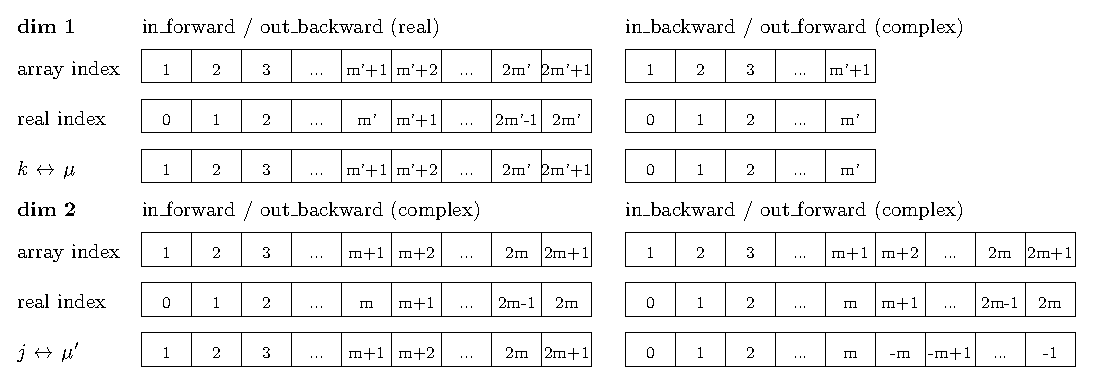
\includegraphics[width=1\textwidth]{_figure/fftw3_indices}
\par\end{center}
\begin{center}
\caption[Indices arrangement in a complete forward-backward FFT-2D process
of m'$\times$m elements]{Indices arrangement in a complete forward-backward \acs{FFT}-2D
process of m'$\times$m elements. The \acs{DFT} of dim 1 ($k$ to
$\mu$) and dim 2 ($j$ to $\mu'$) are done sequentially and \emph{vice
versa}. Array index is the one used by Fortran array, real index is
the one shown in eq. (\ref{eq:fftw3-fwd}) and (\ref{eq:fftw3-bwd}),
$k$ and $j$ indices shown in the left as well as $\mu$ and $\mu'$
in the right are those in eq. (\ref{eq:f_mup_mu}) and (\ref{eq:f_mup_mu_2}).
Here $\mathrm{m}=m_{\mathrm{max}}$ and $\mathrm{m}'=\left\lfloor m_{\mathrm{max}}/s\right\rfloor $.
\label{fig:FFTW3-2D-indices}}
\par\end{center}%
\end{minipage}
\end{figure}

As the output array of FFTW3 is periodic,
\begin{equation}
e^{2\pi i\mu k/n}=e^{2\pi i(\mu-n)k/n}e^{2\pi ik}=e^{2\pi i(\mu-n)k/n}\label{eq:mu-periodicity}
\end{equation}
the indices $\mu=m_{\mathrm{max}}+1,\ldots,2m_{\mathrm{max}}$ actually
correspond to $\mu=-m_{\mathrm{max}},\ldots,-1$. Note that eq. (\ref{eq:f_mup_mu})
and (\ref{eq:f_mup_mu_2}) do not possess the periodicity of eq. (\ref{eq:mu-periodicity}),
only in the domain of definition of $\mu'$ and $\mu$ some intermediary
functions share the same formula with \acs{FFT}.

Moreover, from eq. (\ref{eq:f_mup_mu}), (\ref{eq:f_mup_mu_3}) and
(\ref{eq:symm_f_m_mup_mu}), we can verify that
\begin{equation}
F_{\mu'\mu}(\Theta)=F_{\underline{\mu'}\underline{\mu}}^{*}(\Theta)
\end{equation}
The latter is used in the code since, according to the definition
in eq. (\ref{eq:fftw3-fwd}) and (\ref{eq:fftw3-bwd}), $F_{\underline{\mu'}\underline{\mu}}(\Theta)$
is calculated instead of $F_{\mu'\mu}(\Theta)$.

\section{Operational algorithm\label{sec:Operational-algorithm}}

As described above, the whole process of $\gamma$ and $\mathcal{F}_{\mathrm{exc}}$
functional evaluation proposed by this algorithm can be concluded
as 8 operations:
\begin{enumerate}
\item Firstly, the Fourier transform of the density is computed:
\begin{equation}
\Delta\hat{\rho}(\mathbf{k},\mathbf{\Omega})=\int\mathrm{d}\mathbf{r}\Delta\rho(\mathbf{r},\mathbf{\Omega})e^{-i\mathbf{k}\cdot\mathbf{r}}\label{eq:fft3d-fwd}
\end{equation}
\item Then $\Delta\hat{\rho}(\mathbf{k},\mathbf{\Omega})$ is expanded on
\acs{GSH}s:
\begin{equation}
\Delta\hat{\rho}_{\mu'\mu}^{m}(\mathbf{k})=\frac{f_{m}}{8\pi^{2}}\int\mathrm{d}\mathbf{\Omega}\Delta\hat{\rho}(\mathbf{k},\mathbf{\Omega})R_{\mu'\mu}^{m*}(\mathbf{\Omega})\label{eq:fgsht-fwd}
\end{equation}
Note that these two steps, the same with their backward transform,
are commutable, which will be discussed after.
\item Afterwards the projections in k-frame are then rotated into the local
coordinate system along the unit vector $\mathbf{\hat{k}}$:
\begin{equation}
\Delta\hat{\rho'}_{\chi\mu}^{m}(\mathbf{k})=\sum_{\mu'}\Delta\hat{\rho}_{\mu'\mu}^{m}(\mathbf{k})R_{\mu'\chi}^{m}(\mathbf{\hat{k}})\label{eq:2.2.rho-rot-rho}
\end{equation}
where the rotation matrix elements $R_{\mu'\chi}^{m}(\mathbf{\hat{k}})$
should be calculated directly because of the huge memory required
by its storage. The algorithm by recurrence used to evaluate $R_{\mu'\chi}^{m}(\mathbf{\hat{k}})$
in this thesis is detailed in appendix \ref{chpt:rotM-by-recurrence}.
\item Next, computing the OZ equation with Blum's reduction:
\begin{equation}
\hat{\gamma'}_{\chi\mu}^{m}(\mathbf{k})=\sum_{n,\nu}(-1)^{\chi+\nu}\hat{c'}_{\mu\nu,\chi}^{mn}(\mathbf{k})\Delta\hat{\rho'}_{\chi\underline{\nu}}^{n}(\mathbf{k})\label{eq:OZ-2}
\end{equation}
\item The $\gamma$ projections are then transformed back to global coordinates
system:
\begin{equation}
\hat{\gamma}_{\mu'\mu}^{m}(\mathbf{k})=\sum_{\chi}\hat{\gamma'}_{\chi\mu}^{m}(\mathbf{k})R_{\mu'\chi}^{m*}(\mathbf{\hat{k}})
\end{equation}
\item From here the function in angular frame can thus be rebuilt:
\begin{equation}
\hat{\gamma}(\mathbf{k},\mathbf{\Omega})=\sum_{m,\mu',\mu}f_{m}\hat{\gamma}_{\mu'\mu}^{m}(\mathbf{k})R_{\mu'\mu}^{m}(\mathbf{\Omega})\label{eq:fgsht-bwd}
\end{equation}
\item Then the inverse Fourier transform of these projections is:
\begin{equation}
\gamma(\mathbf{r},\mathbf{\Omega})=\int\mathrm{d}\mathbf{k}\hat{\gamma}(\mathbf{k},\mathbf{\Omega})e^{i\mathbf{r}\cdot\mathbf{k}}
\end{equation}
\item Finally, the functional $\mathcal{F}_{\mathrm{exc}}$ is computed
by:
\begin{equation}
\mathcal{F}_{\mathrm{exc}}=-\frac{k_{\mathrm{B}}T}{2}\int\mathrm{d}\mathbf{r}\mathrm{d}\mathbf{\Omega}\Delta\rho(\mathbf{r},\mathbf{\Omega})\gamma(\mathbf{r},\mathbf{\Omega})
\end{equation}
\end{enumerate}

\subsection{Commutativity between operations\label{subsec:Commutativity-between-operations}}

As mentioned in the operational algorithm, three types of operations
are being done before and after the \acs{OZ} equation. They are:
\begin{enumerate}
\item Fast Fourier transform for 3-dimensional spatial grid (\acs{FFT}3D):
implemented by package FFTW3 \citep{FFTW3}, mathematically leading
to no accuracy loss;
\item Fast generalized spherical harmonics transform (\acs{FGSHT}): has
real or complex input, is exact if $F(\mathbf{\Omega})$ can be given
as an expansion of \acs{GSH}s of order at most $m_{\mathrm{max}}$;
\item Rotation between laboratory coordinate system and local system linked
to vector $\mathbf{k}$ (RotS): can be done for both function and
projections. It introduces a minus error in accuracy at origin and
border of the box, which will be discussed in $\mathsection$\ref{subsec:k-border-effect}.
\end{enumerate}
Their commutativity is shown in figure \ref{fig:Commutativity-of-operations}.

\begin{figure}[h]
\begin{centering}
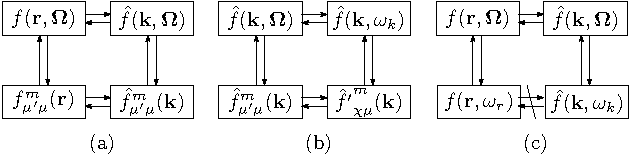
\includegraphics{_figure/algorithms_commutativity}
\par\end{centering}
\caption[Commutativity of operations]{Commutativity of operations. (a) FFT3D and FGSHT; (b) RotS and FGSHT;
(c) FFT3D and RotS.\label{fig:Commutativity-of-operations}}
\end{figure}

As shown in figure \ref{fig:Commutativity-of-operations}, the \acs{FFT}3D
does not depend on the angular part of the function, and the \acs{FGSHT}
does not depend on the spatial part of the function. The two operations
are commutative. 

It can be also proven that the passage from the function $\hat{f}$
in laboratory frame $\hat{f}(\mathbf{k},\mathbf{\Omega})$ to the
projections in local frame ${f'}_{\chi\mu}^{m}(\mathbf{k})$ can be
achieved either by a rotation to the function $\hat{f}(\mathbf{k},\boldsymbol{\omega}_{k})$
in intermolecular frame following by an \acs{GSH} expansion as eq.
(\ref{eq:gamma-projection-local}), or an \acs{GSH} expansion that
gives the projections $f_{\mu'\mu}^{m}(\mathbf{k})$ following by
a rotation as eq. (\ref{eq:gamma-p}).

However, the rotation from $f(\mathbf{r},\mathbf{\Omega})$ to $f(\mathbf{r},\boldsymbol{\omega})$
depends on the vector $\mathbf{r}$, of which the information is totally
lost after \acs{FFT}3D. The rotation from $f(\mathbf{k},\mathbf{\Omega})$
to $f(\mathbf{k},\boldsymbol{\omega})$ can only depend on the vector
$\mathbf{k}$; they are not the same rotation, therefore non-commutative. 

\subsection{Reduction by symmetry\label{subsec:Reduction-by-symmetry}}

A further reduction of computing cost can be made by performing about
only half of the operations, thanks to the symmetric relations between
the projections.

In eq. (\ref{eq:fgsht-fwd}), $\Delta\rho(\mathbf{r},\mathbf{\Omega})$
is real. With the property of \acs{GSH} (eq. (\ref{eq:symm-gsh-1})):
\begin{equation}
R_{\mu'\mu}^{m}(\mathbf{\Omega})=(-)^{\mu'+\mu}R_{\underline{\mu'}\underline{\mu}}^{m*}(\mathbf{\Omega})
\end{equation}
we find
\begin{equation}
\Delta\hat{\rho}_{\mu'\mu}^{m}(\mathbf{r})=(-)^{\mu'+\mu}\Delta\hat{\rho}_{\underline{\mu'}\underline{\mu}}^{m*}(\mathbf{r})\label{eq:2.2.symm-rho-r}
\end{equation}
Therefore only the projections of $\mu'\geq0$ or $\mu\geq0$ are
needed to generate all information.

When $\Delta\hat{\rho}_{\mu'\mu}^{m}(\mathbf{r})$ is transformed
into $k$-space, replacing
\begin{equation}
\Delta\hat{\rho}_{\mu'\mu}^{m}(\mathbf{k})=\int\mathrm{d}\mathbf{r}\Delta\rho_{\mu'\mu}^{m}(\mathbf{r})e^{-i\mathbf{r}\cdot\mathbf{k}}
\end{equation}
 with eq. (\ref{eq:2.2.symm-rho-r}) gives
\begin{equation}
\Delta\hat{\rho}_{\mu'\mu}^{m}(\mathbf{k})=(-)^{\mu'+\mu}\Delta\hat{\rho}_{\underline{\mu'}\underline{\mu}}^{m*}(-\mathbf{k})\label{eq:2.2.symm-rho-k}
\end{equation}
Therefore only the projections of $\mu'\geq0$, $\mu\geq0$, or a
half of $\mathbf{k}$ where one of the dimensions $k_{i}\geq0$ are
independent. 

In the implementation, it is a natural choice to keep only a half
of projections $\Delta\hat{\rho}_{\mu'\mu}^{m}(\mathbf{k})$, as either
the real-to-complex \acs{FFT}3D ($k_{3}\geq0$) or the real-to-complex
\acs{FGSHT} ($\mu\geq0$) gives implicitly a half of information.
As the \acs{OZ} equation (\ref{eq:gamma-blum}) is separable for
each $\mathbf{k}$, but not on $\mu$ ($\nu$ in equation), it is
more natural compute a half of $\mathbf{k}$, which is actually the
choice in our code. All the rest we should prove is that the $\hat{\gamma}_{\mu'\mu}^{m}(\mathbf{k})$
calculated from this half of known density is still able to generate
all the informations.

The relation deduced from the symmetries of \acs{GSH} (appendix \ref{chpt:symmetry}):
\begin{equation}
r_{\mu'\mu}^{m}(\theta)=(-)^{m+\mu'}r_{\mu'\underline{\mu}}^{m}(\pi-\theta)
\end{equation}
\begin{eqnarray}
R_{\mu'\mu}^{m}(\phi\theta\psi) & = & (-)^{m+\mu'}e^{i\mu'\pi}R_{\mu'\underline{\mu}}^{m}(\pi+\phi,\pi-\theta,-\psi)\\
 & = & (-)^{m}R_{\mu'\underline{\mu}}^{m}(\pi+\phi,\pi-\theta,-\psi)
\end{eqnarray}
gives that
\begin{equation}
R_{\lambda'0}^{l}(\hat{\mathbf{k}})=(-)^{l}R_{\lambda'0}^{l}(-\hat{\mathbf{k}})=(-)^{l+\lambda'}R_{\underline{\lambda'}0}^{l*}(-\hat{\mathbf{k}})\label{eq:2.2.symm-lambda}
\end{equation}

If we replace eq. (\ref{eq:im}) by eq. (\ref{eq:2.2.symm-rho-k})
and (\ref{eq:2.2.symm-lambda}), with symmetry of 3j-symbol (\ref{eq:symm-3j-symbol})
and symmetry of $\hat{c}$ \citep{Blum_I}:
\begin{equation}
\hat{c}_{\mu\nu}^{mnl}(k)=\left(-\right)^{m+n+\mu+\nu}\hat{c}_{\underline{\mu}\underline{\nu}}^{mnl*}(k)
\end{equation}
we have the same symmetry property for $\hat{\gamma}$ as for $\Delta\hat{\rho}$:
\begin{equation}
\hat{\gamma}_{\mu'\mu}^{m}(\mathbf{k})=\left(-\right)^{\mu'+\mu}\hat{\gamma}_{\underline{\mu'}\underline{\mu}}^{m*}(-\mathbf{k})
\end{equation}
which means the half $\hat{\gamma}_{\mu'\mu}^{m}(\mathbf{k})$ is
sufficient to generate $\hat{\gamma}(\mathbf{k},\mathbf{\Omega})$
or $\gamma(\mathbf{r},\mathbf{\Omega})$. Thus the \acs{OZ} equation
can be safely reduced by a factor of two. 

We can also find
\begin{equation}
R_{\mu'\chi}^{m}(\hat{\mathbf{k}})=(-)^{m}R_{\mu'\underline{\chi}}^{m}(-\hat{\mathbf{k}})=(-)^{m+\mu'+\chi}R_{\underline{\mu'}\chi}^{m}(-\hat{\mathbf{k}})\label{eq:3}
\end{equation}
which gives
\begin{equation}
\Delta\hat{\rho'}_{\chi\mu}^{m}(\mathbf{k})=(-)^{m+\mu+\chi}\Delta\hat{\rho'}_{\chi\underline{\mu}}^{m*}(-\mathbf{k})
\end{equation}
\begin{equation}
\hat{\gamma'}_{\chi\mu}^{m}(\mathbf{k})=(-)^{m+\mu+\chi}\hat{\gamma'}_{\chi\underline{\mu}}^{m*}(-\mathbf{k})
\end{equation}

If we replaced the \acs{OZ} equation by these two equations, we can
find the symmetries of $\hat{c'}_{\mu\nu,\chi}^{mn}(k)$ in eq. (\ref{eq:rot-invar-symm-k-chi}):
\begin{equation}
\hat{c}_{\mu\nu,\chi}^{mn}(k)=\left(-\right)^{m+n+\mu+\nu}\hat{c}_{\underline{\mu}\underline{\nu},\chi}^{mn*}(k)
\end{equation}

It should be noted that not exactly the half of points are calculated.
If we choose to calculate a half of $\mathbf{k}$, as shown in figure
\ref{fig:points-symm}, where the 2D plan corresponds two of the three
dimensions in $k$-space grid, the green points can be generated from
the black points by the symmetries of eq. (\ref{eq:2.2.symm-rho-k}),
but the red points should be all calculated, of which the corresponding
points is also a red point or even itself. This ever caused a huge
problem in the implementation, as we put $\Delta\hat{\rho}_{\mu'\mu}^{m}(\mathbf{k})$
and $\hat{\gamma}_{\mu'\mu}^{m}(\mathbf{k})$ in the same array for
reason of memory. It should be assured that these points are calculated
only once.

\begin{figure}[th]
\begin{centering}
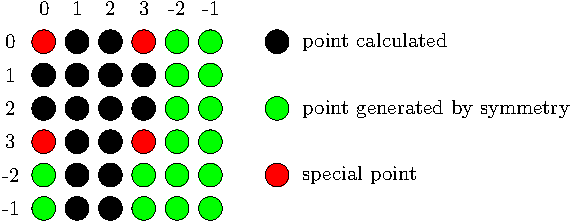
\includegraphics{_figure/test_lmn}
\par\end{centering}
\caption{Distribution of points to be calculated according to symmetry in a
2D plan\label{fig:points-symm}}
\end{figure}

